
\chapter{绪论}
\label{chap:introduction}

Transformer\cite{vaswani2017attention}是一种利用自注意力机制处理序列数据的文本建模模型。自从BERT \cite{devlin2018bert}开始,各种基于Transformer的模型与变种模型已经在各种自然语言处理任务上取得了一波又一波的冲击,包括语言模型\cite{child2019generating,kitaev2020reformer}、翻译\cite{lewis2019bart}、摘要\cite{qi2020prophetnet}、文本分类\cite{he2020deberta}、问答\cite{lan2019albert,beltagy2020longformer,dai2020funnel}等等,都有基于Transformer的模型取得了同期最佳的结果。

Transformer的成功,可部分归功于其自注意力机制,这种机制在序列,即句子的所有token两两之间计算一个分数,以更好地在整个序列中传递、汇总信息。因此,时间和空间复杂度与序列长度的平方成正比。在文本较短时尚可接受,但对于长文本任务来说,自注意力机制就会带来巨大的时间与内存开销。因此,BERT和很多基于Transformer的模型都将一次计算的序列长度限制在512个token\cite{cohan2018discourse}。而对于文本远长于512的数据集(比如arXiv,见\autoref{table.sum_data}),这种限制无疑会降低模型的表现。而这种限制也体现在问答、长文本分类等其他任务上。为了把长文本的输入长度限制在512,可以采取分割成长度为512的片段的办法,但这样会丢失片段间的关联,为了弥补这种丢失又会使模型更加复杂。

\begin{figure}
\centering
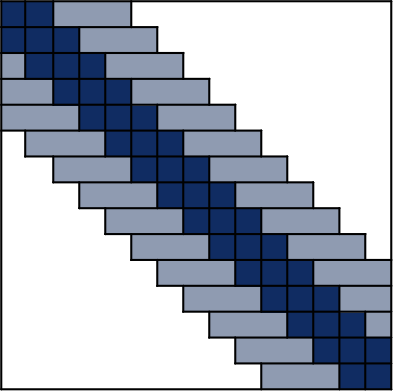
\includegraphics[width=0.5\textwidth]{pfarch}
\caption{Poolingformer 的双层注意力机制示意图。每列、行分别对应query、key序列的一个token,涂色代表着对应的两个token要计算注意力。深色为第一层注意力的接收窗口,浅色为第二层注意力的接收窗口,相连的格子表示对应的token序列经过池化操作,被压缩为一个token。}
\label{fig:pfarch}
\end{figure}

为了解决这个问题,在现有工作\cite{beltagy2020longformer,zaheer2020big,miculicich2018document}的基础上,本文提出了Poolingformer,它将Transformer的完全的自注意力机制改为了一种双层的稀疏注意力机制。在第一层里,token只和部分token计算自注意力,这部分token包括所有的全局token和自己相邻的一定长度的窗口内的的token。而全局token 和全部的token 计算自注意力,总体上是一种滑动窗口的自注意力。这一层与Longformer\cite{beltagy2020longformer}的自注意力是一样的。在此之上的第二层里,每个token关注范围是更大的相邻窗口,为了减少关注的token数量,将窗口对应的token序列进行池化操作,每个token与池化后的序列计算注意力。\autoref{fig:pfarch}形象展示了Poolingformer的双层注意力机制。与只有第一层自注意力的模型\cite{beltagy2020longformer,zaheer2020big}相比,Poolingformer的第二层注意力能让token接受到更大范围的token,这就意味着更加丰富的信息。和Transformer相比,Poolingformer 的双层稀疏注意力在分层利用信息上做的更好,将算力按照信息的重要程度分配,最关键的信息能够获得最密集的算力,而非Transformer的完全的自注意力机制那样将算力平均分配,在长文本的情景下能够大量的节约运算力资源。Poolingformer的时间和空间复杂度只与序列长度成线性关系。

与此同时,本文还将Poolingformer与Deberta——另外一个基于Transformer的模型相结合。Deberta\cite{he2020deberta}改进了token位置信息的融入方式,采用了一种新的相对位置编码,在短文本理解的任务上取得了同期最佳的结果。由于两种模型修改了Transformer的两个不同的要素,因此将Poolingformer的注意力计算模式,与Deberta的自注意力分数计算,两者结合起来,用于长文本理解的任务,应该会得到一个更好的结果。
